\chapter{Modell}
\label{chp:modell}

Im ersten Schritt soll die digitale Modellierung des zu erschaffenden Mars Rovers erfolgen.
Dazu wird gemäß der Spezifikation die Anwendung BrickLink-Studio in der Version 2.0.10 genutzt.
Diese ermöglicht die umfangreiche und präzise Modellierung mit LEGO-Elementen sowie beispielsweise Funktionen zur Stabilitätsanalyse und Generierung schrittweiser Bauanleitungen.
In den folgenden drei Abschnitten sind jeweils eine gerenderte Front- und Seitenansicht und eine Draufsicht des Mars-Rover-Modells dargestellt.
Zusätzlich ist zum Vergleich in jedem Abschnitt eine Fotografie des realen Modells aus der entsprechenden Perspektive abgebildet.

\section{Vorderansicht}
\label{sec:voderansicht}

\begin{figure}
	\centering
	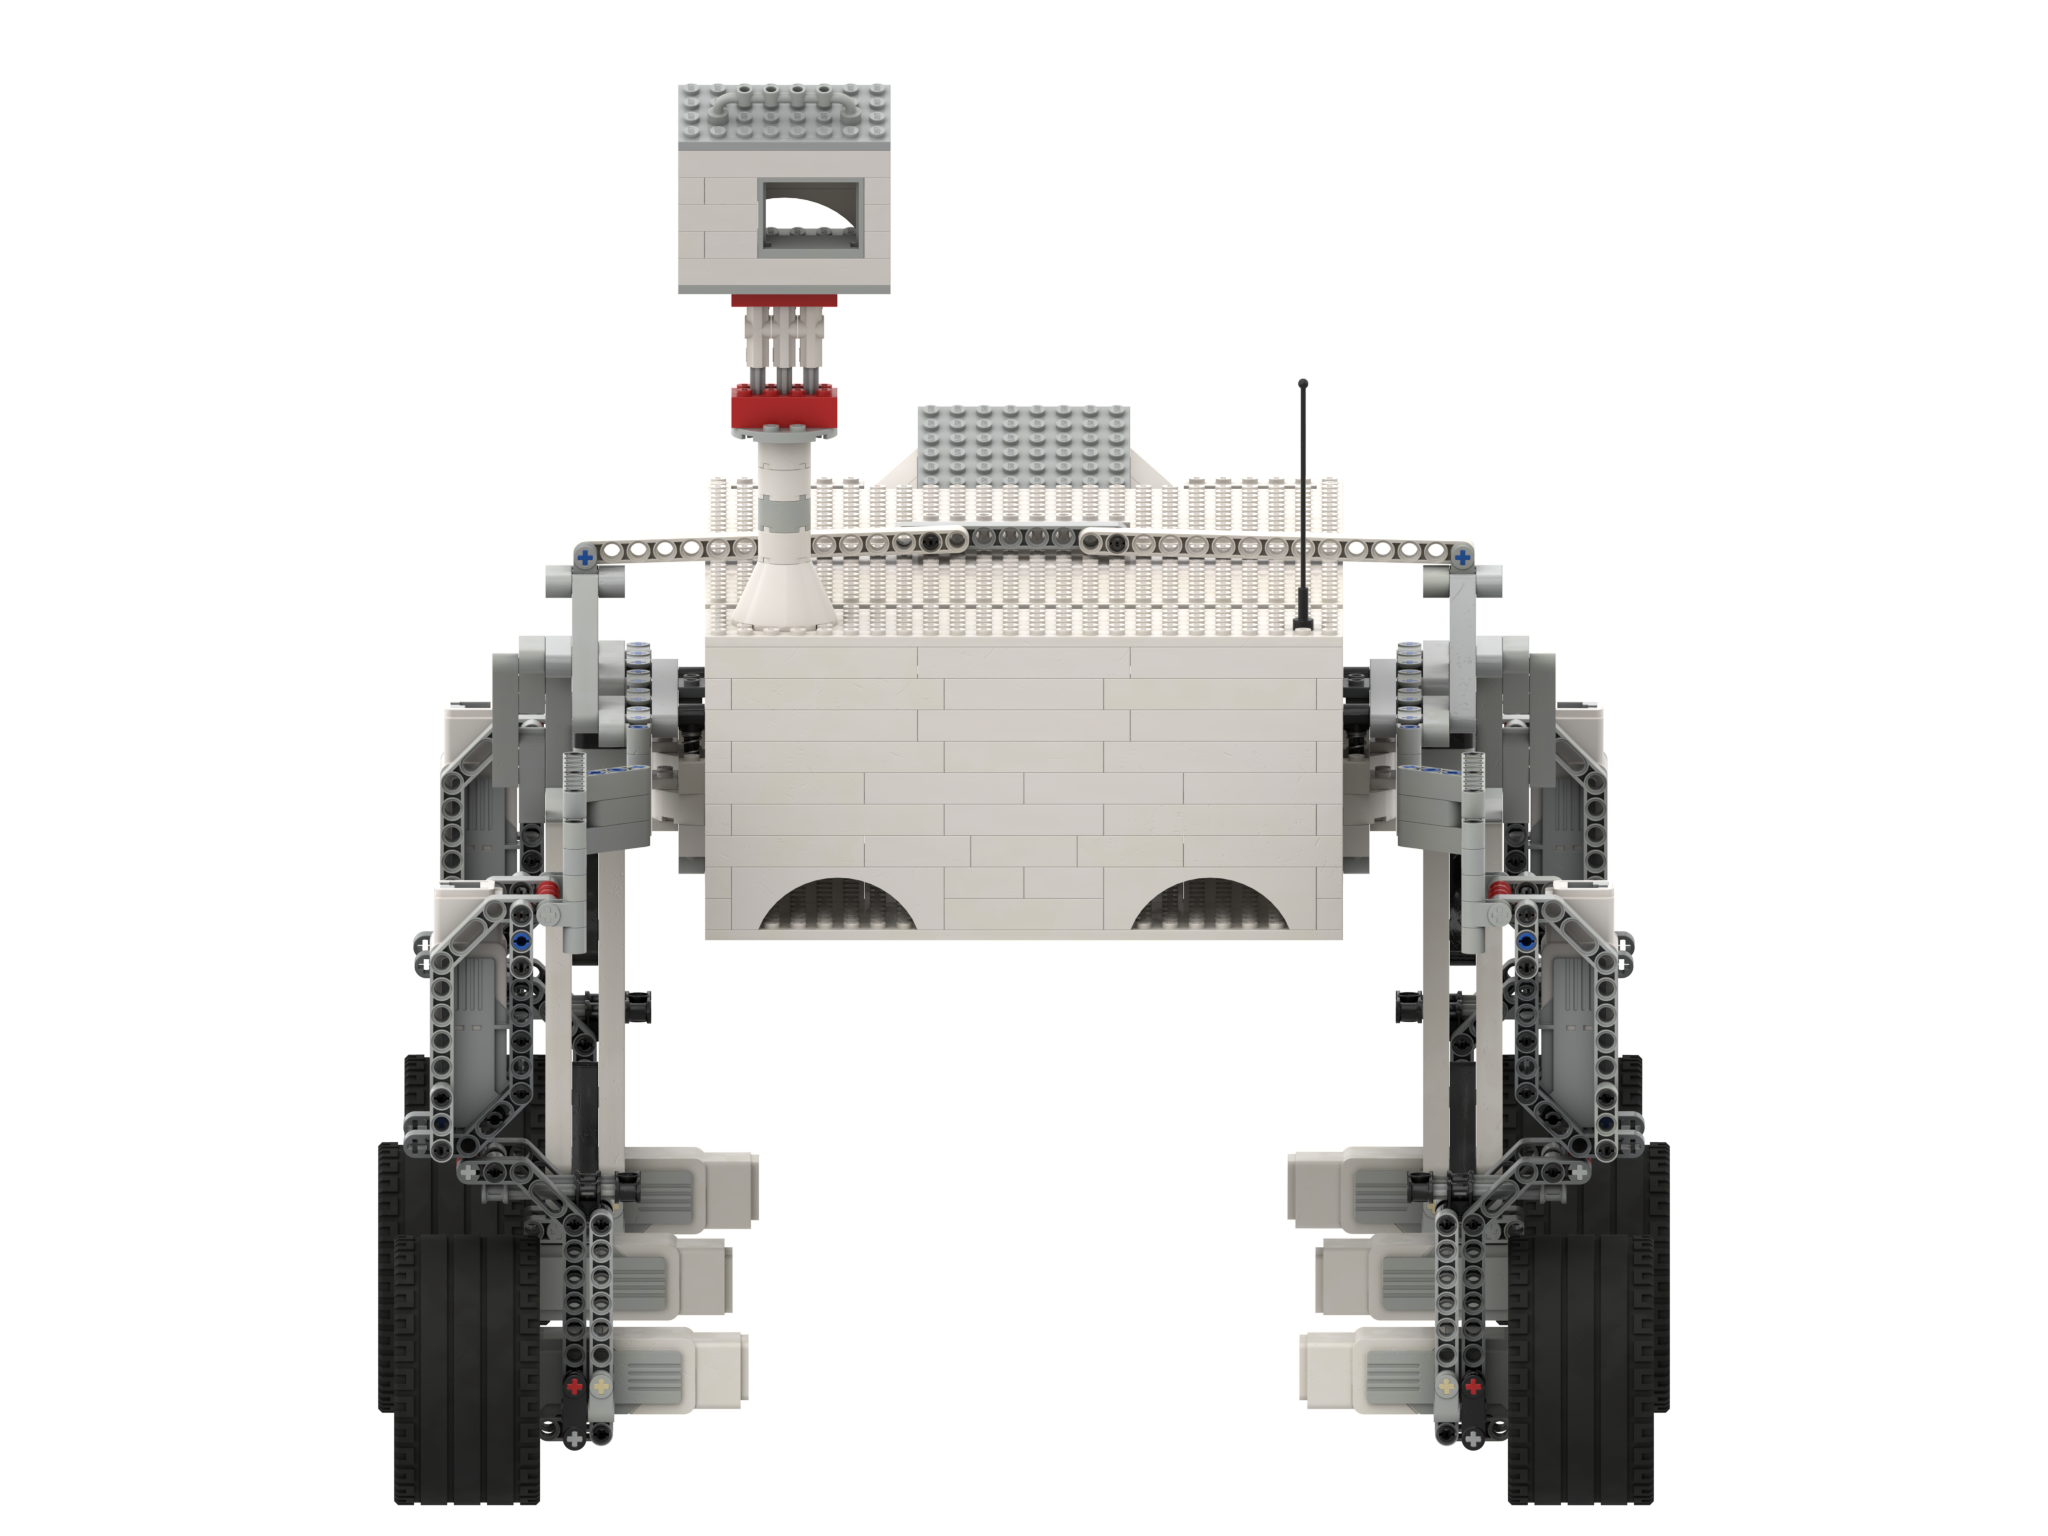
\includegraphics[width=\textwidth]{../Images/20200429_Mars_Rover_V5_front.png}
	\vspace{0.5em}
	\parbox[c]{0.8\linewidth}{\footnotesize
		\centering
		\vspace{1em}
		Quelle: eigene Darstellung (Render-Export aus BrickLink Studio 2.0.10)
	}
	\caption{Gerenderte Frontansicht des digitalen Rover-Modells}
	\label{fig:roverfrontrender}
\end{figure}

\begin{figure}
	\centering
	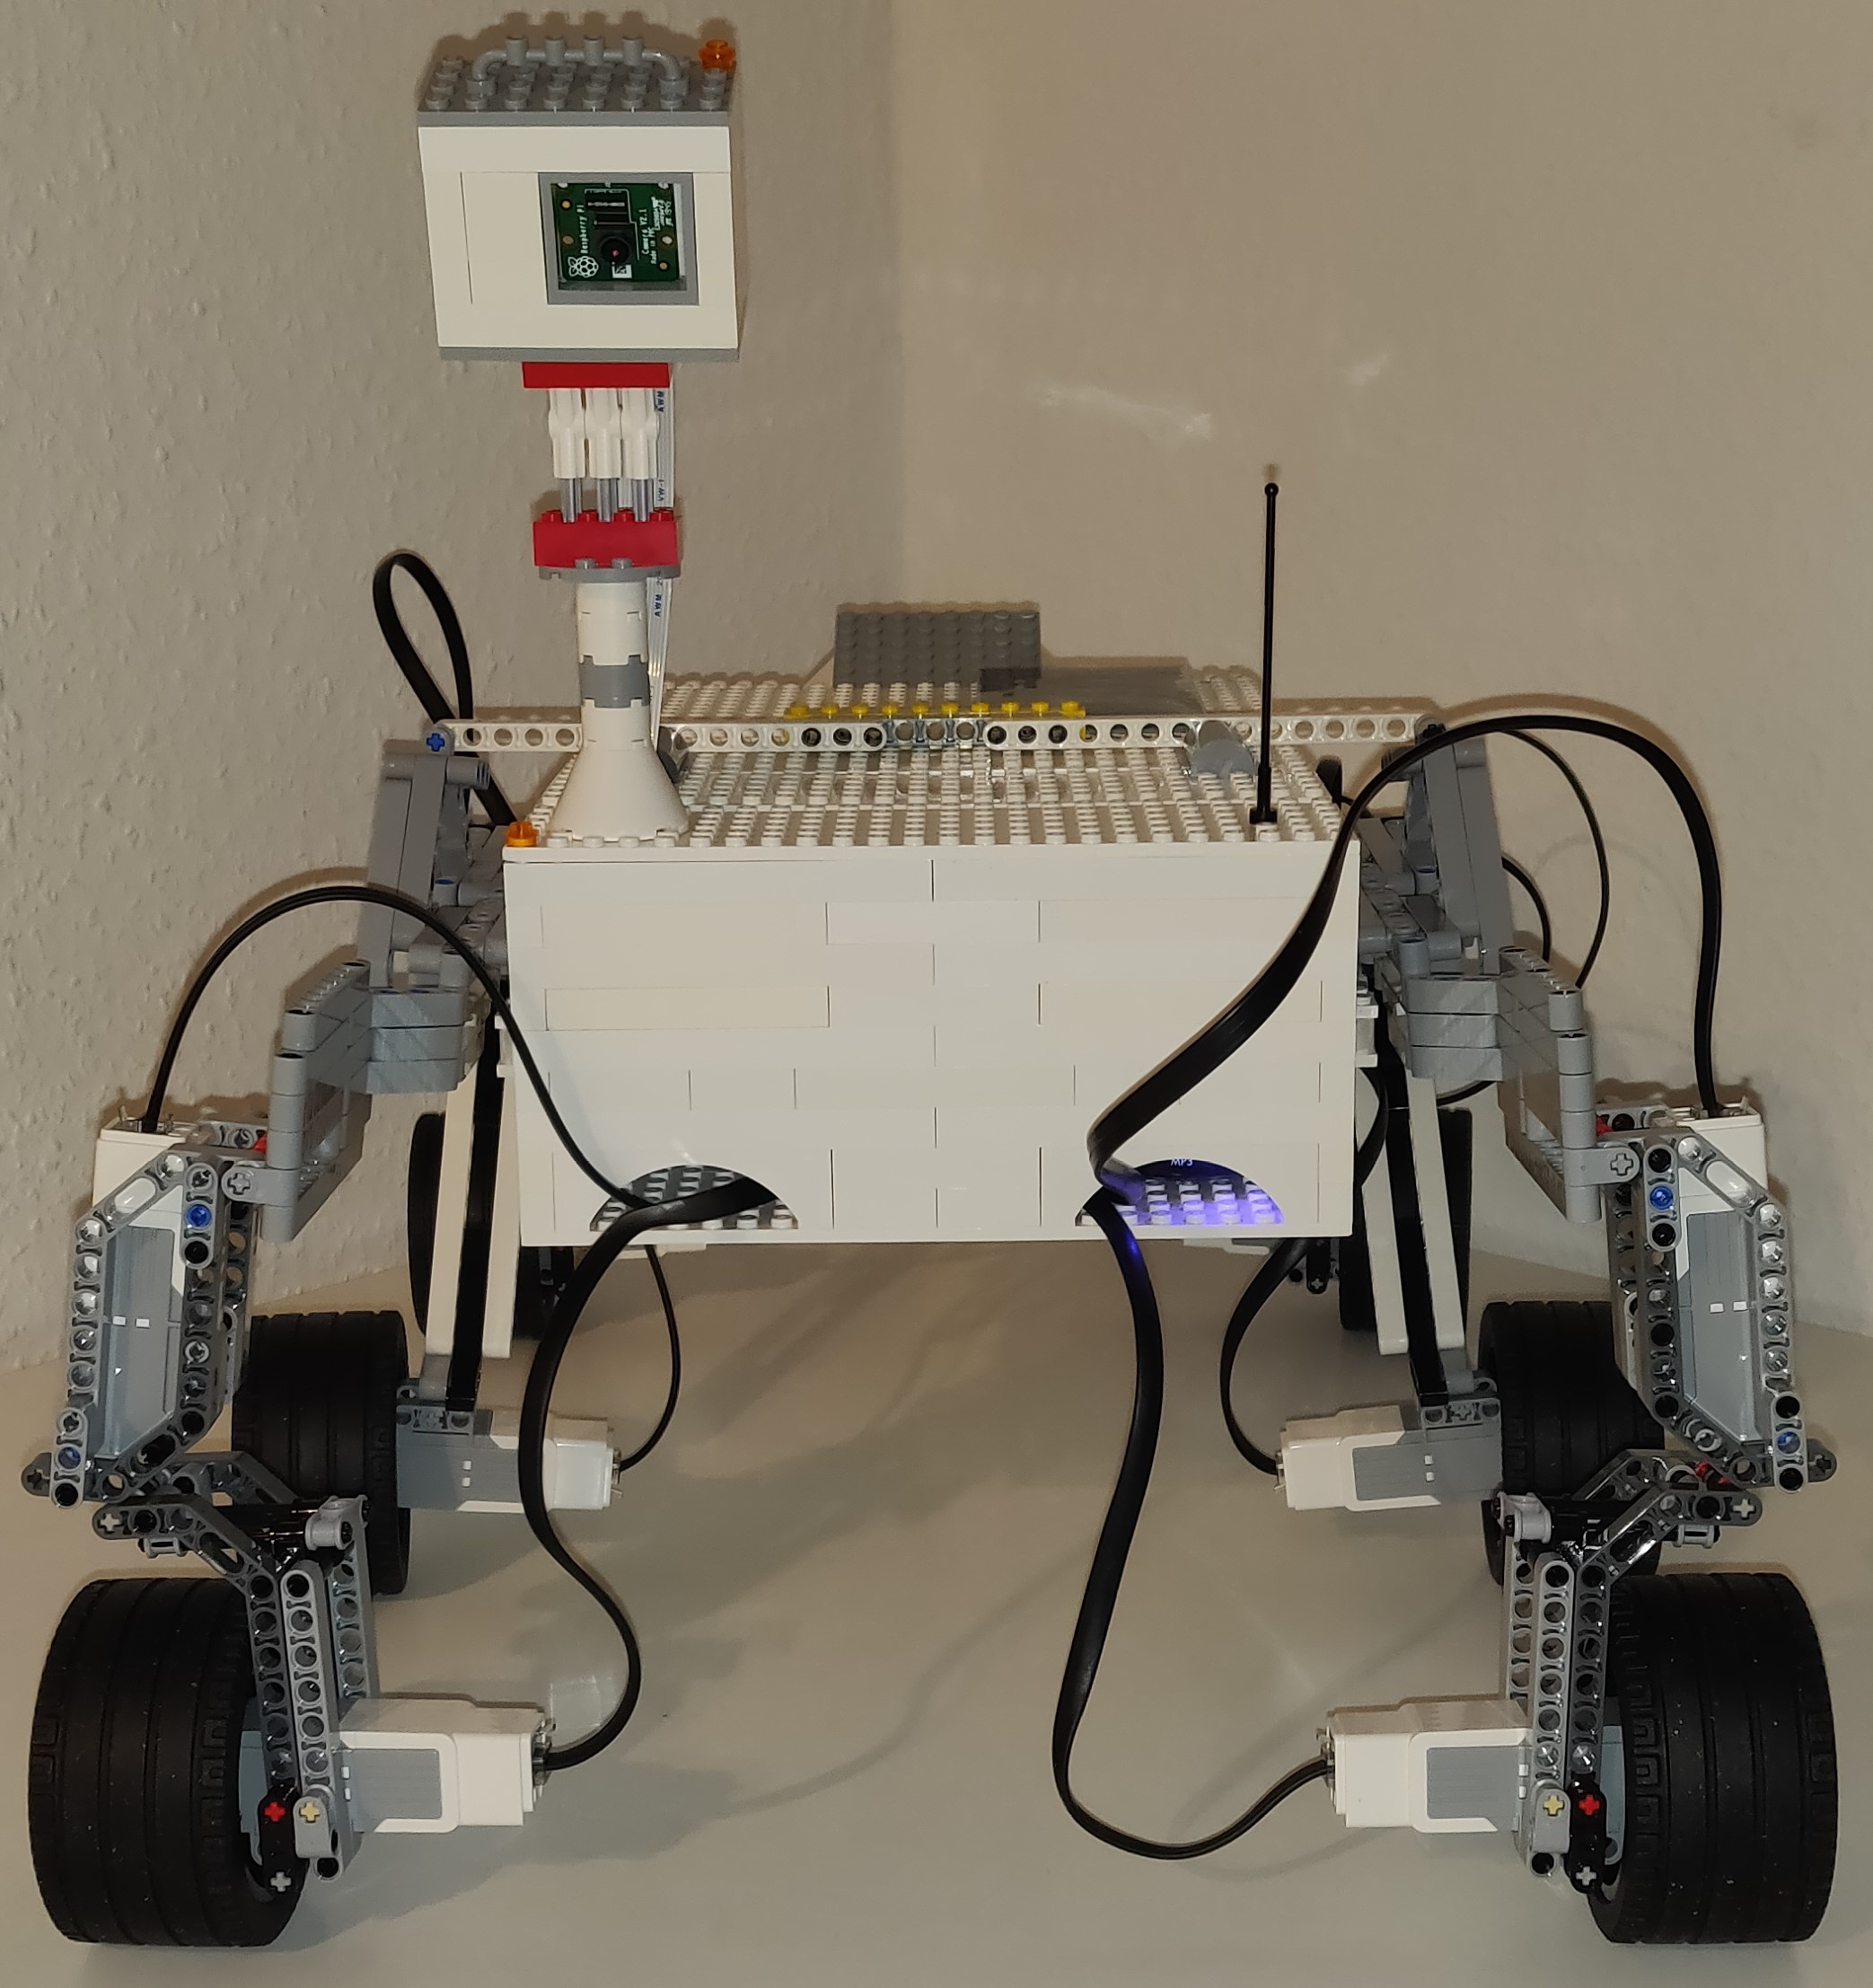
\includegraphics[width=\textwidth]{../Images/20200429_front_01.jpg}
	\vspace{0.5em}
	\parbox[c]{0.8\linewidth}{\footnotesize
		\centering
		\vspace{1em}
		Quelle: eigene Aufnahme
	}
	\caption{Fotografie des realen Rover-Modells aus Frontansicht}
	\label{fig:roverfrontfoto}
\end{figure}

In der Frontalansicht sind die zwei breiten Vorderräder, die über jeweils einen Motor zum Antrieb und einen für die Lenkung des Rades verfügen, zu erkennen.
Über eine Aufhängung sind sie mit dem Korpus des Rovers verbunden und etwas von diesem abgesetzt, um die Stabilität zu erhöhen.
Weiterhin ist in der Realaufnahme die genutzte Kamera (siehe dazu Abschnitt \ref{sec:inst_konf_kamera}), platziert im charakteristischen Kopf des Rovers, erkennbar.
Der Kopf ist um $22{,}5 \degree$ nach unten geneigt, sodass die Erkennung von Wasserobjekten auch auf kurze Distanz möglich bleibt.
Durch die beiden Öffnungen an der Unterkante des Korpus sind die Verbindungskabel zu den vorderen Motoren verlegt.

\section{Seitenansicht}
\label{sec:seitenansicht}

\begin{figure}
	\centering
	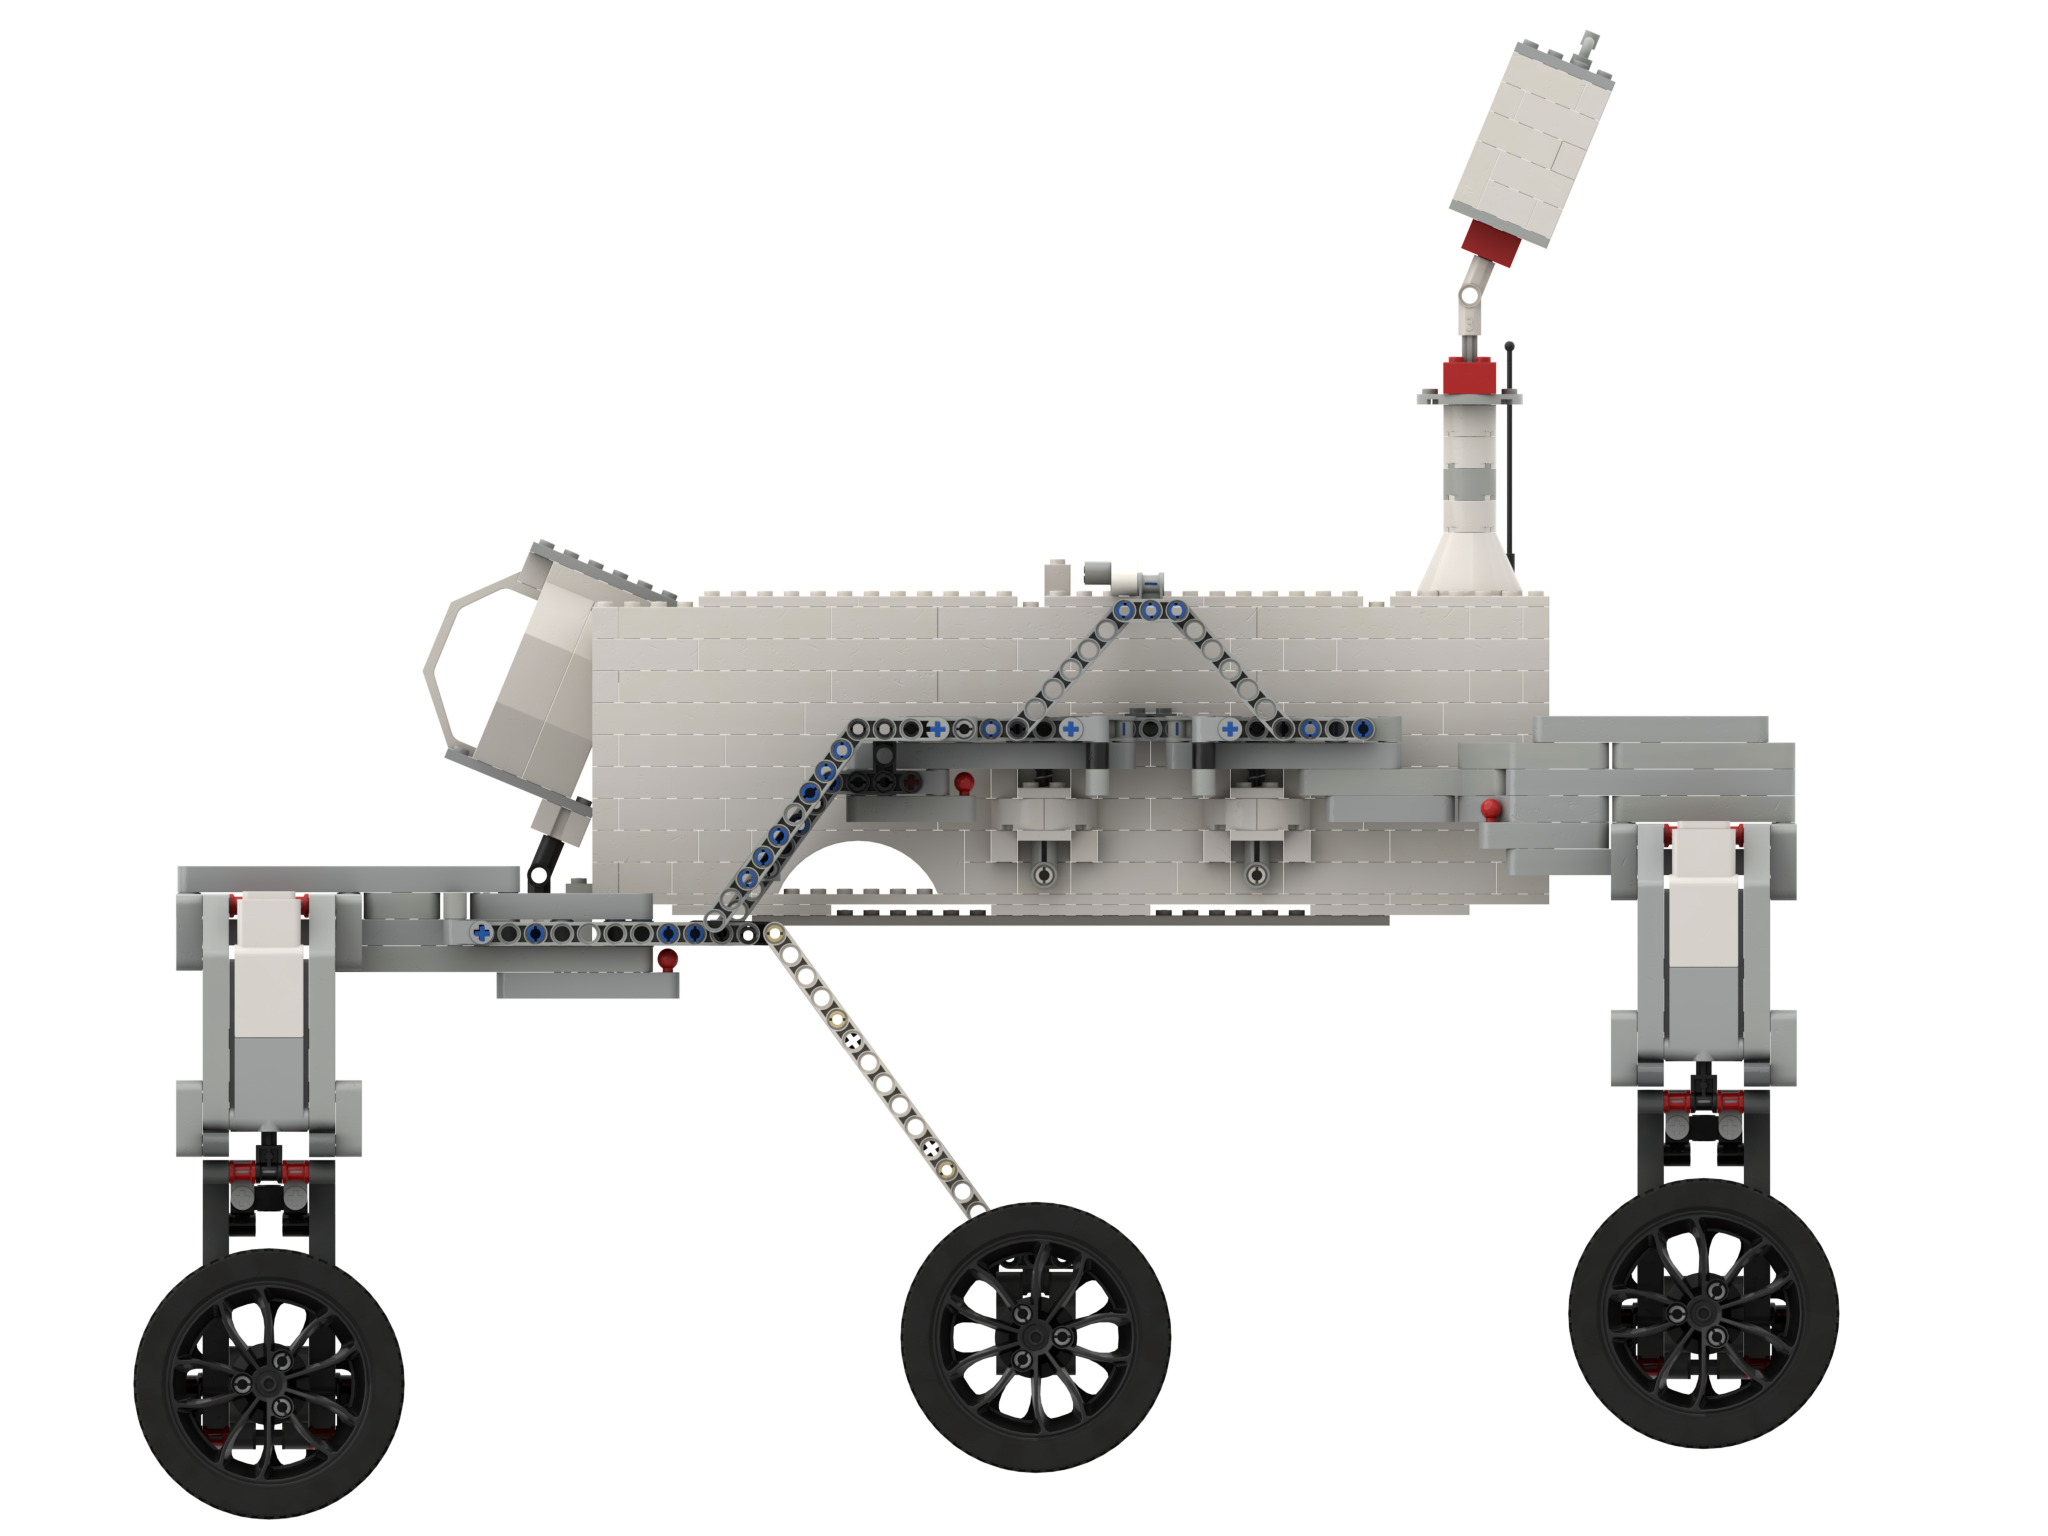
\includegraphics[width=\textwidth]{../Images/20200429_Mars_Rover_V5_side.png}
	\vspace{0.5em}
	\parbox[c]{0.8\linewidth}{\footnotesize
		\centering
		\vspace{1em}
		Quelle: eigene Darstellung (Render-Export aus BrickLink Studio 2.0.10)
	}
	\caption{Gerenderte Seitenansicht des digitalen Rover-Modells}
	\label{fig:roversiderender}
\end{figure}

\begin{figure}
	\centering
	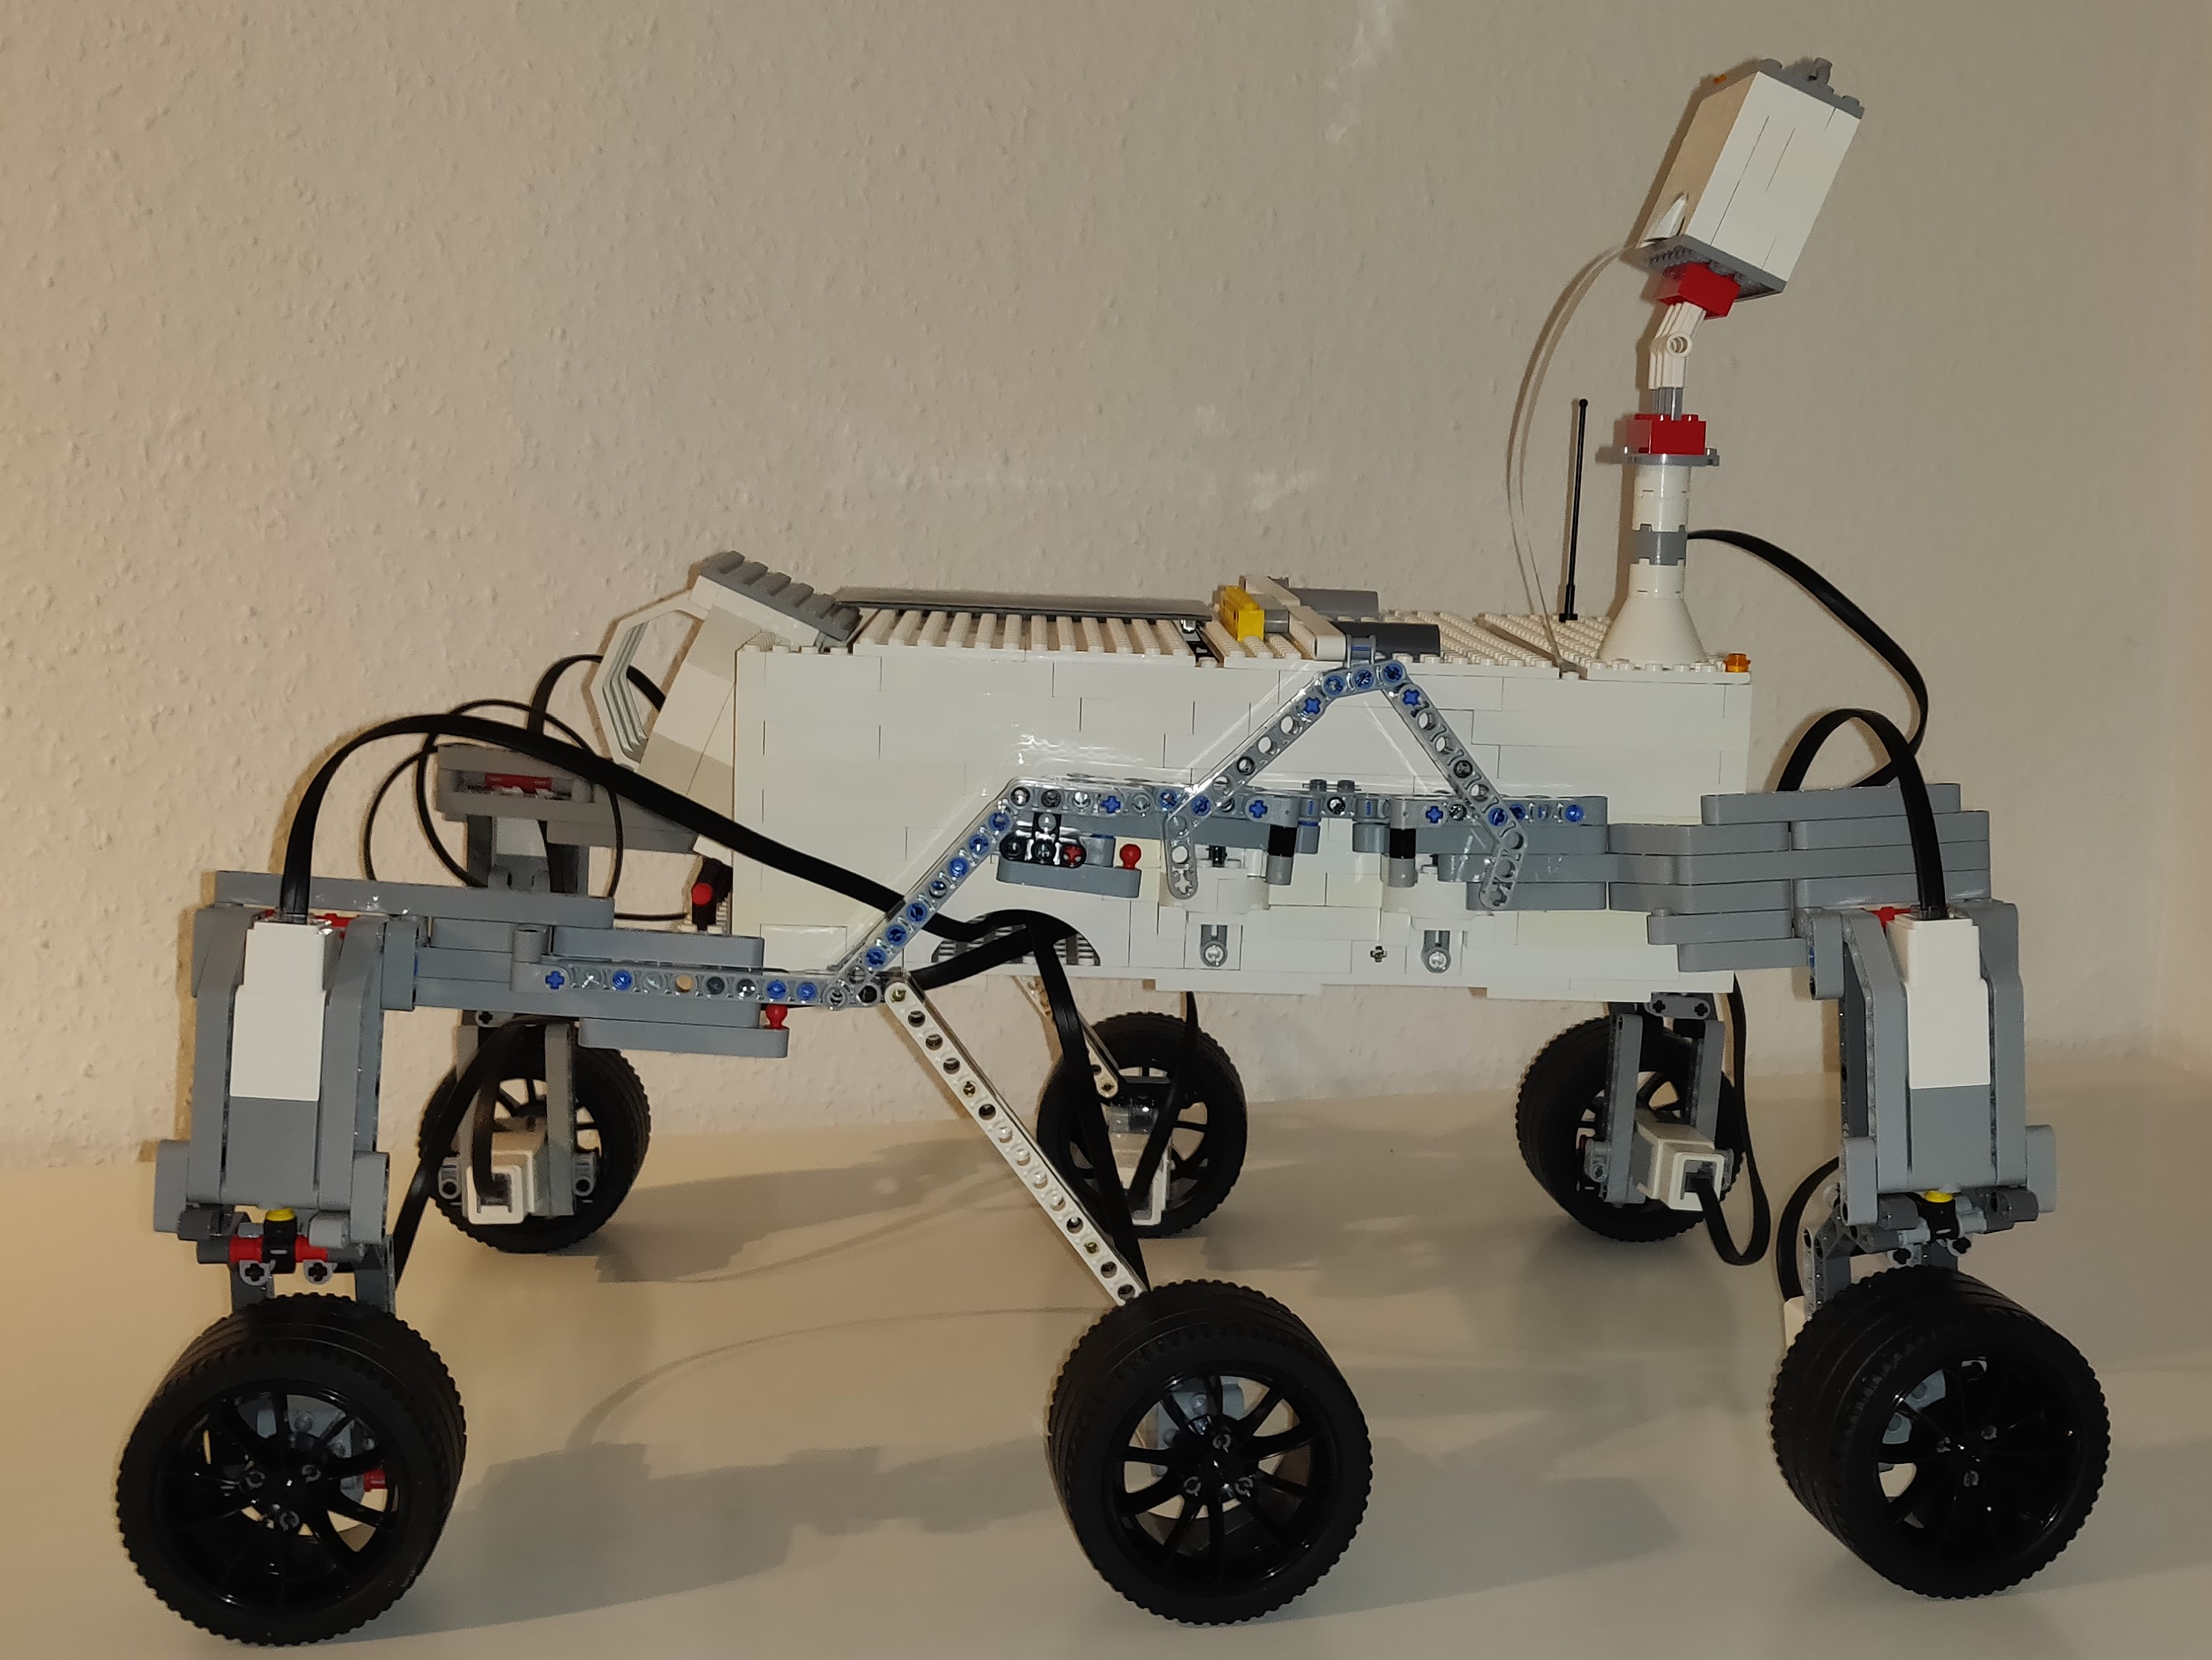
\includegraphics[width=\textwidth]{../Images/20200429_side_01.jpg}
	\vspace{0.5em}
	\parbox[c]{0.8\linewidth}{\footnotesize
		\centering
		\vspace{1em}
		Quelle: eigene Aufnahme
	}
	\caption{Fotografie des realen Rover-Modells aus Seitenansicht}
	\label{fig:roversidefoto}
\end{figure}

Der im vorherigen Abschnitt beschriebene Neigungswinkel des Kopfes wird in der Seitenansicht deutlich.
Weiterhin sind die mittleren und hinteren Räder des Rovers zu sehen.
Auf beiden Seiten sind diese starr miteinander und gemeinsam wiederum an einem einzigen Punkt mit einer vom Korpus ausgehenden, gefederten Strebe verbunden.
Dies entspricht dem Aufbau des Rocker-Bogie-Systems, welches bei Curiosity zum Einsatz gekommen ist.
So ist sichergestellt, dass die mittleren Räder, die den Rover seitlich stabilisieren und antreiben, sowie die hinteren Räder, die ihn antreiben und gegebenenfalls lenken, in jedem Fall den Bodenkontakt beibehalten.
Bezüglich der Verbindung zum Korpus wurde vom Rocker-Bogie-System insofern abgewichen, dass dieser nicht frei um einen Punkt rotieren kann, da eine kontrollierte Verlagerung seines Schwerpunkts entlang der Fahrtrichtungsachse aktuell nicht ermöglicht werden kann.
Entsprechend bestünde zum Beispiel durch Reibung an der Verbindungsstelle zur Aufhängung oder Windeinwirkung von vorn oder hinten die Gefahr, dass der Korpus kippt und nicht selbsttätig zurückgedreht werden kann.
Es ist jedoch eine minimale Drehung um den zentralen Ankerpunkt zwischen Korpus und Fahrwerk möglich. 
Durch zwei Federn, die an beiden Seiten auf gleicher Höhe zu diesem Punkt angebracht sind, wird der Korpus wenn nötig zurück in die Waagerechte gefedert.

Die Öffnungen links der Ankerpunkte dienen hier auch der Kabelführung, in diesem Fall für die Kabel zu den mittleren und hinteren Motoren.

\section{Ansicht von oben}
\label{sec:draufsicht}

\begin{figure}
	\centering
	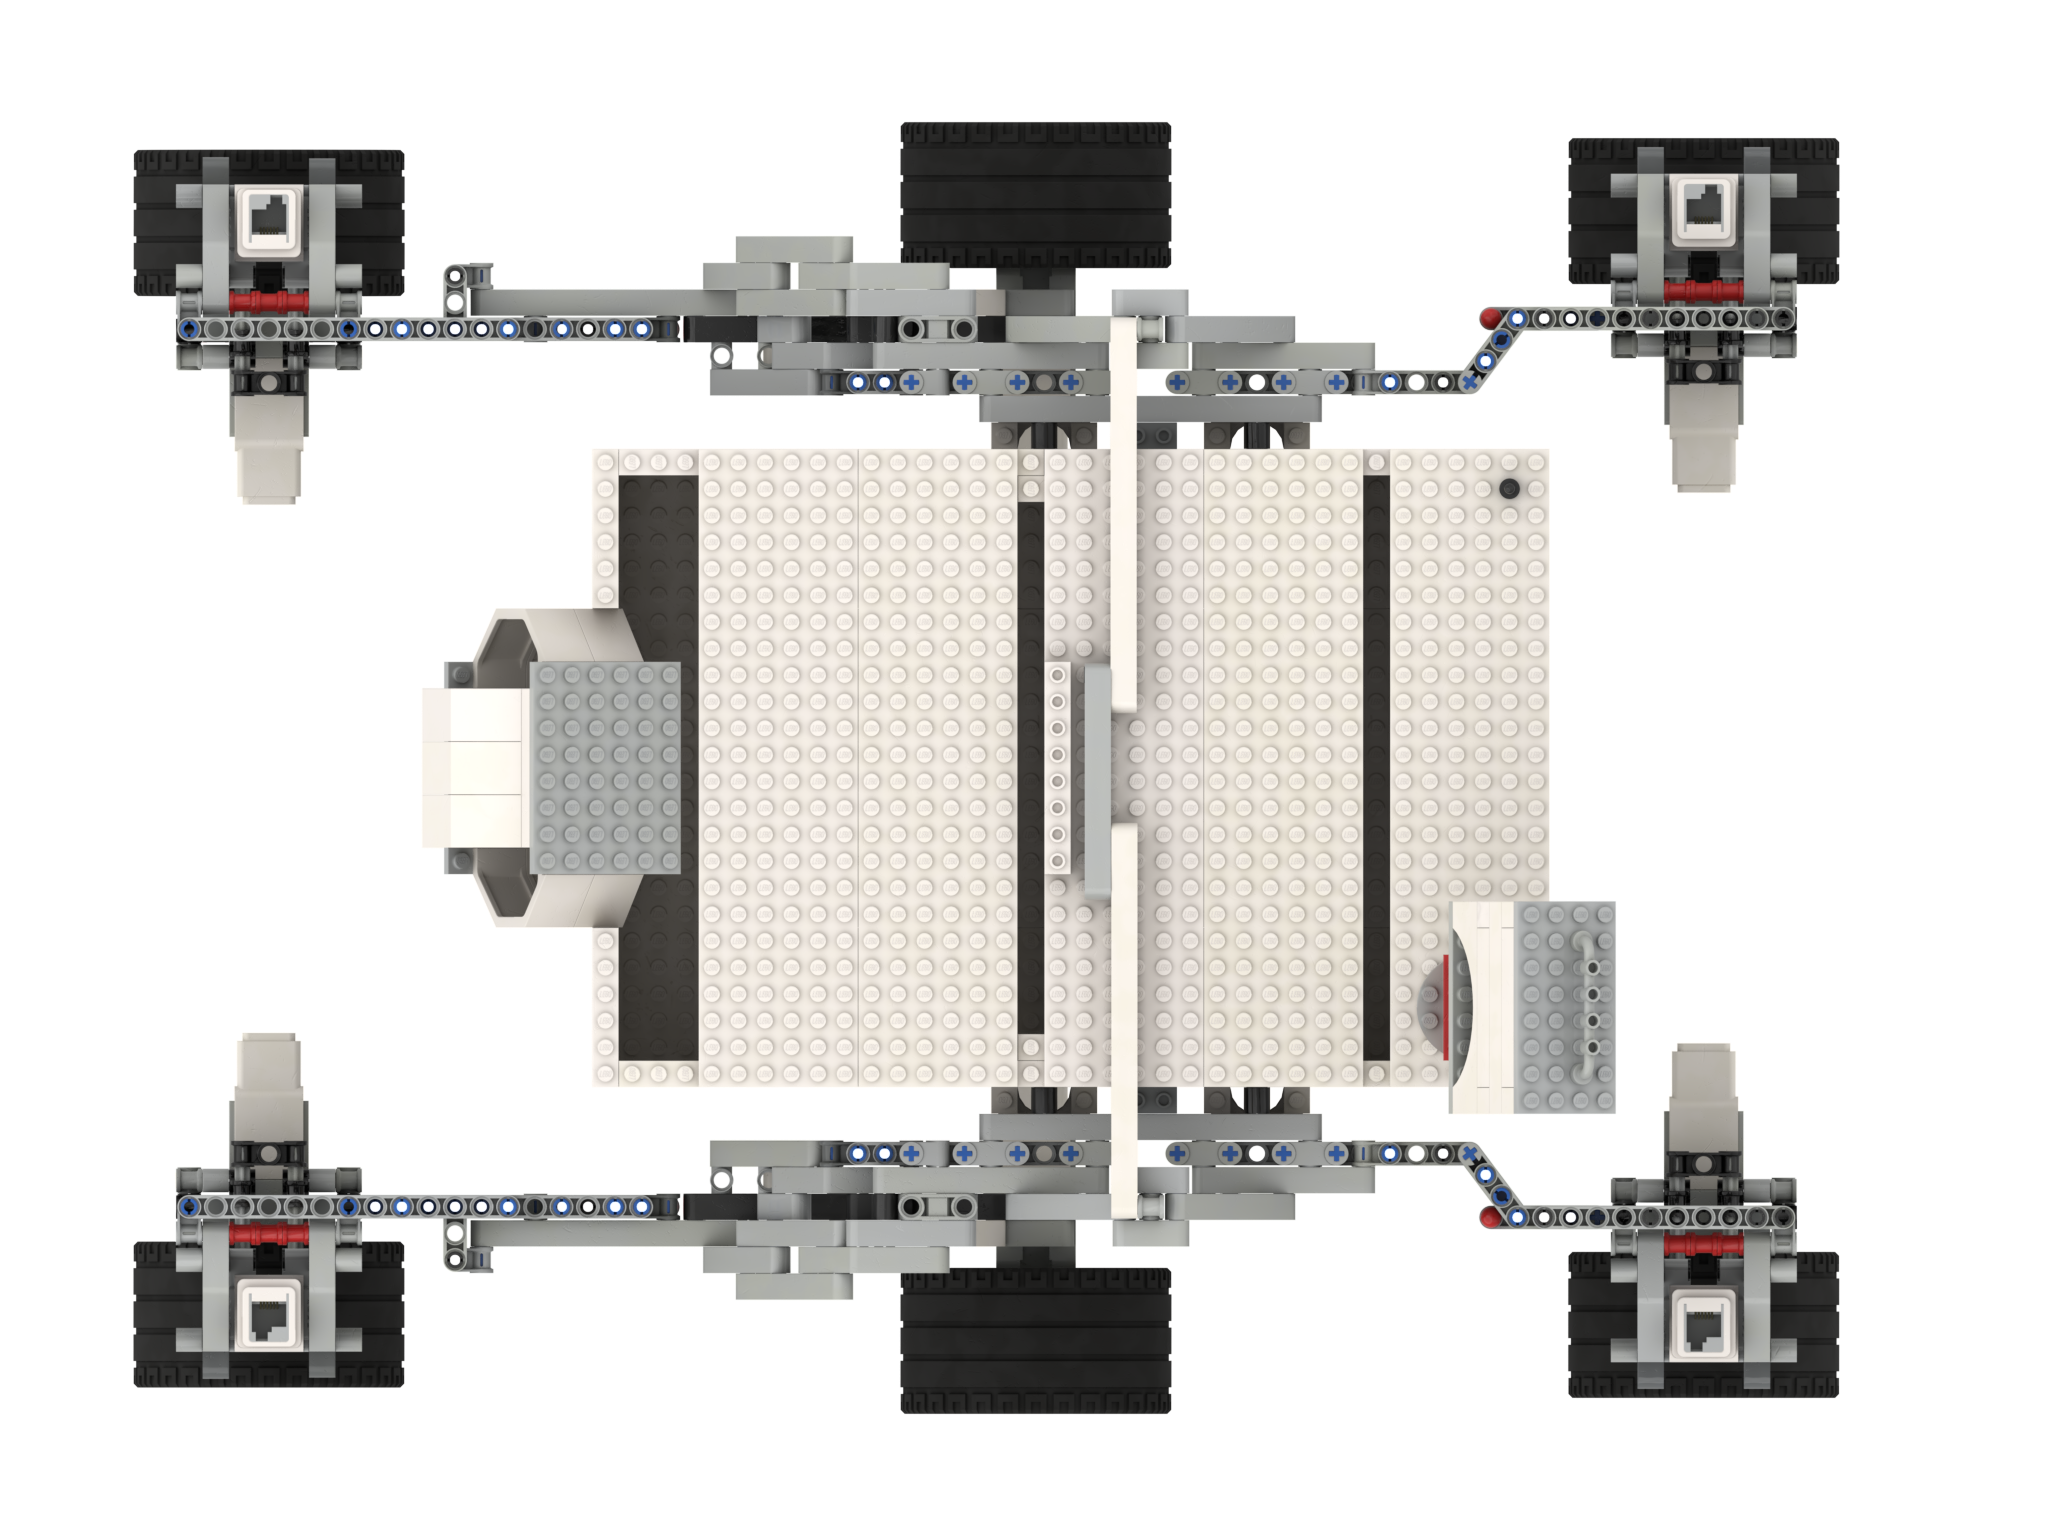
\includegraphics[width=\textwidth]{../Images/20200429_Mars_Rover_V5_top.png}
	\vspace{0.5em}
	\parbox[c]{0.8\linewidth}{\footnotesize
		\centering
		\vspace{1em}
		Quelle: eigene Darstellung (Render-Export aus BrickLink Studio 2.0.10)
	}
	\caption{Gerenderte Draufsicht des digitalen Rover-Modells}
	\label{fig:rovertoprender}
\end{figure}

\begin{figure}
	\centering
	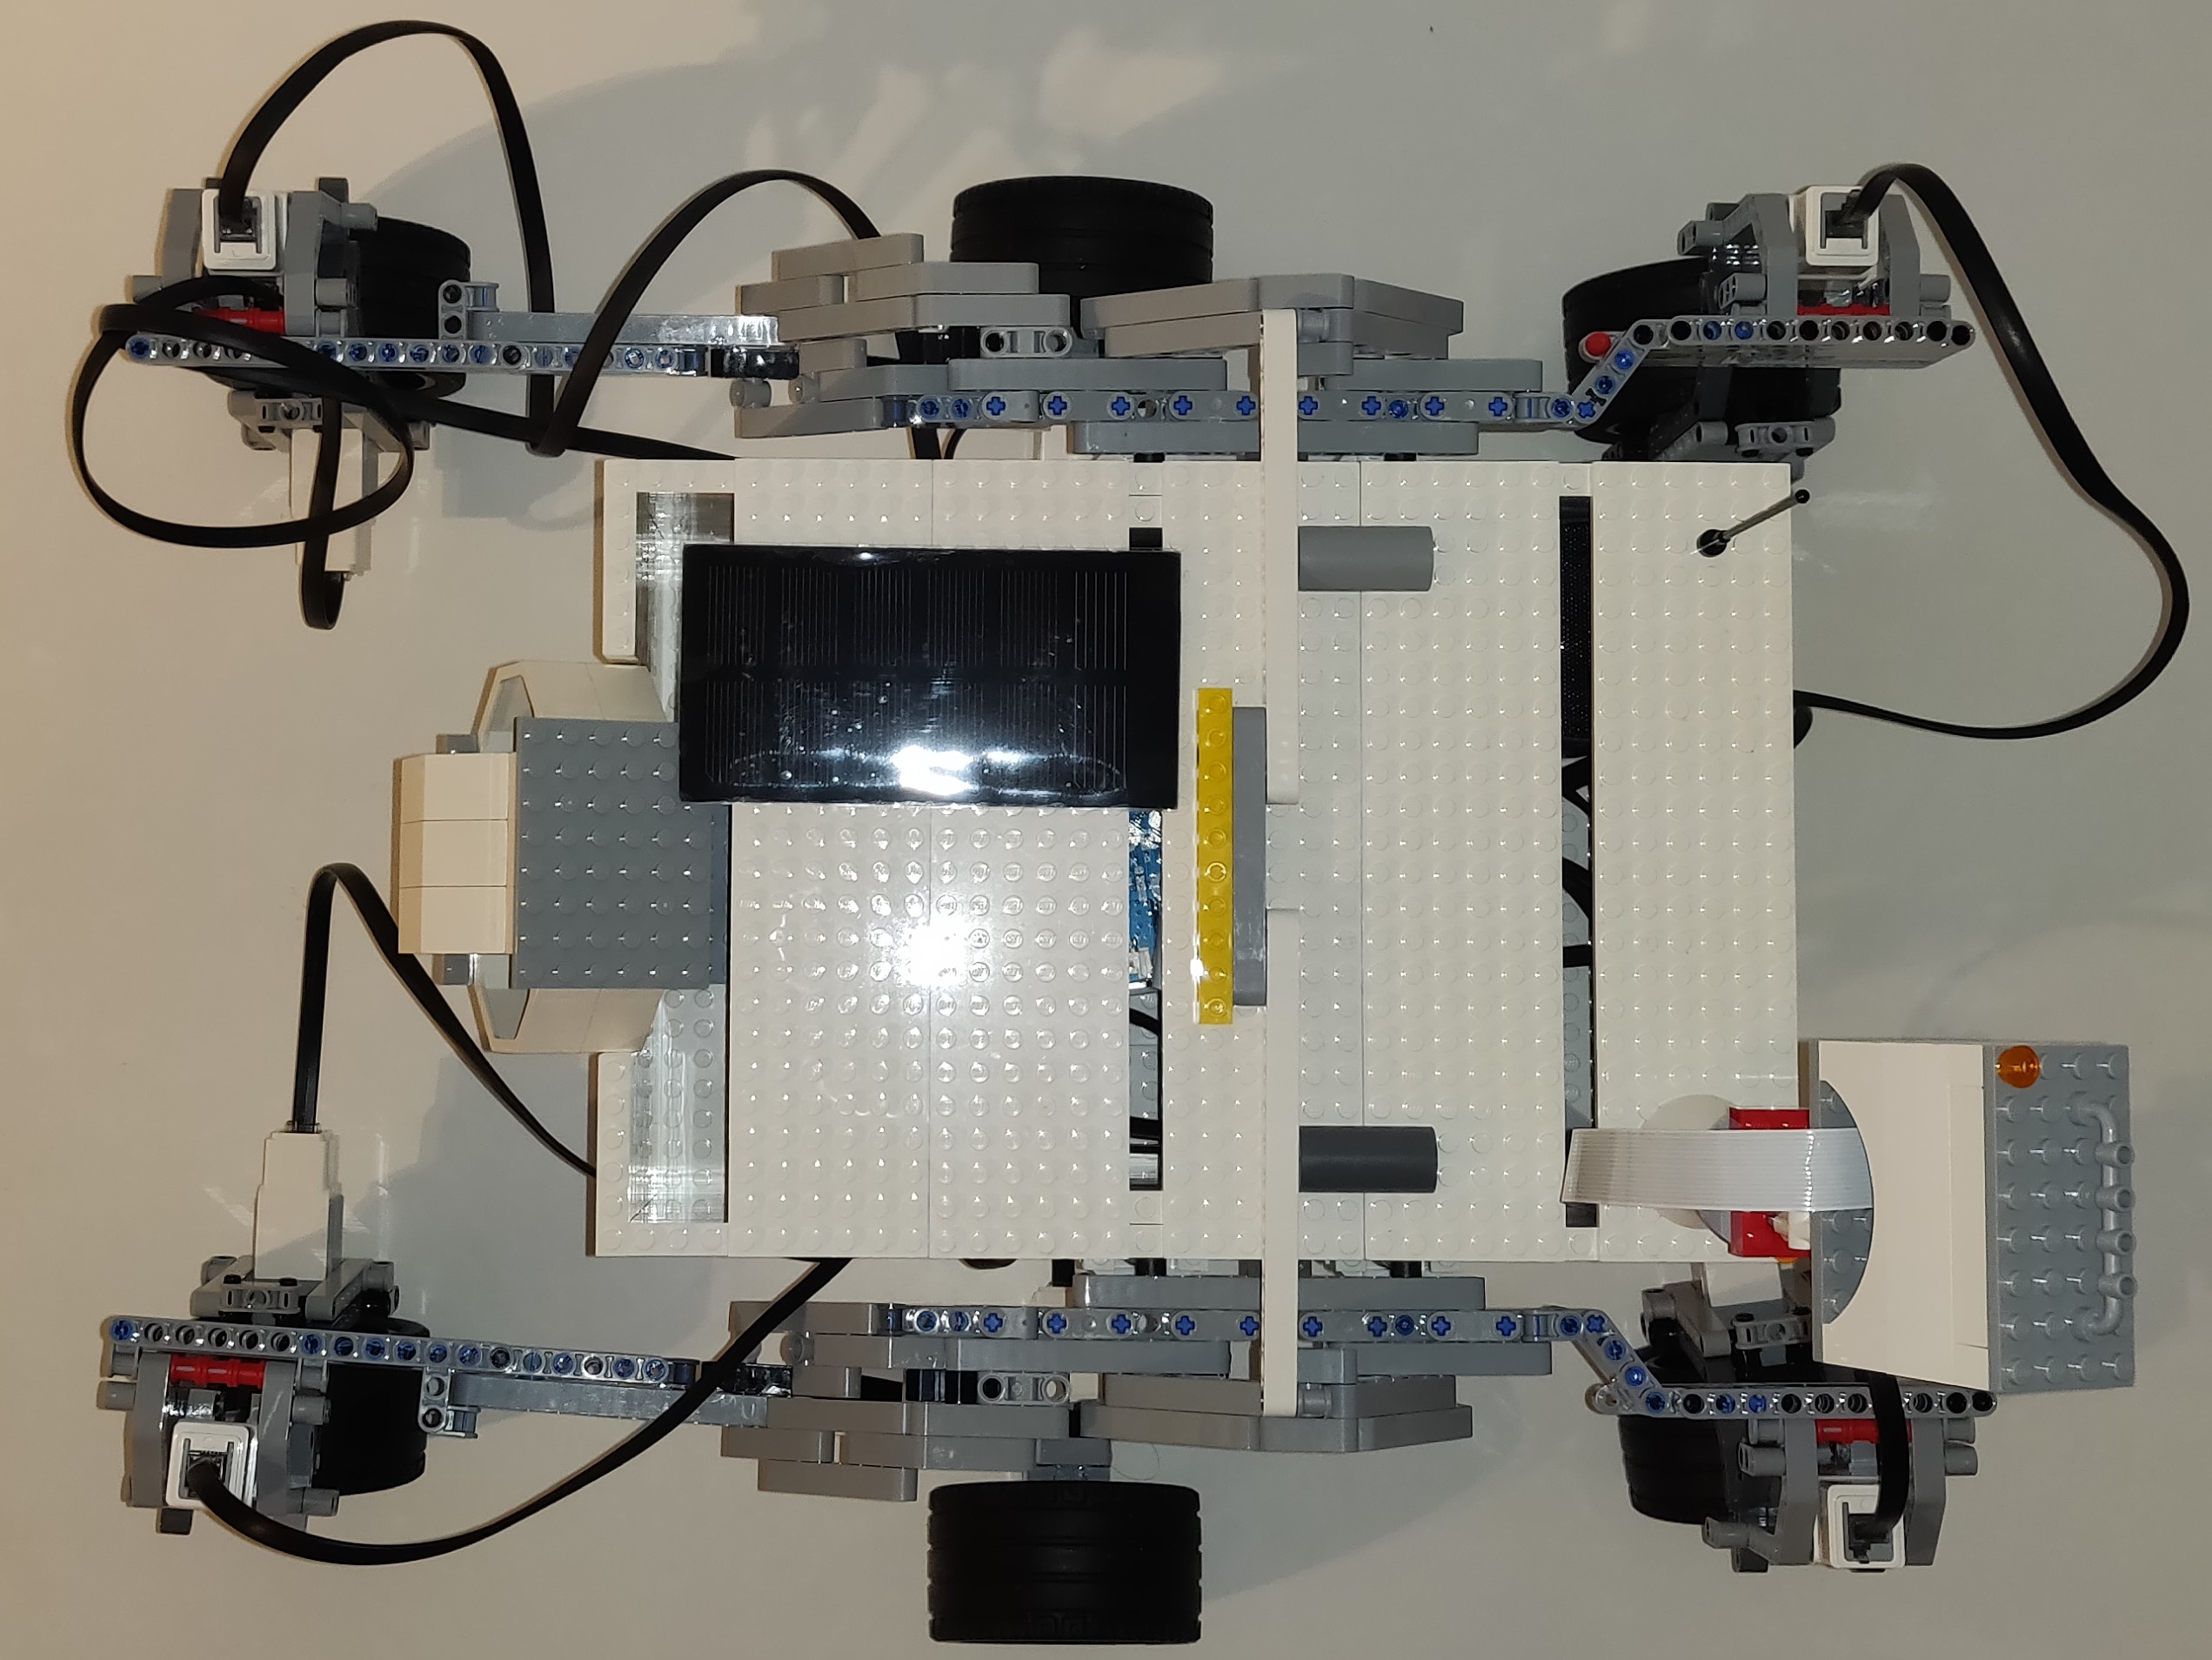
\includegraphics[width=\textwidth]{../Images/20200429_top_01.jpg}
	\vspace{0.5em}
	\parbox[c]{0.8\linewidth}{\footnotesize
		\centering
		\vspace{1em}
		Quelle: eigene Aufnahme
	}
	\caption{Fotografie des realen Rover-Modells aus Draufsicht}
	\label{fig:rovertopfoto}
\end{figure}

In der Draufsicht ist ein aus einigen Liftarm-Streben bestehender, brückenartiger Überbau auf dem Rover zu erkennen.
Dieser dient einerseits der gleichmäßigeren Lastverteilung und unterstützt andererseits die Ankerpunkte zwischen Korpus und Fahrwerk, da die Teile dauerhaft unter Spannung stehen und dadurch seitlich von außen Druck auf die Ankerpunkte ausüben.
Im digitalen Modell ist die Strebe in der Mitte dieses Überbaus asymmetrisch zum Rest, da BrickLink Studio es nicht ermöglicht, die Teile unter Spannung anzubringen.
Die Fotografie des realen Modells zeigt, wie die Anbringung konzipiert ist, und dass die diagonal angeordneten Streben an den Ankerpunkten (in Abbildung \ref{fig:rovertopfoto} oben und unten mittig) zur Mitte gezogen werden.

Bei Betrachtung des realen Modells von oben erkennt man das Solarpaneel auf dem Korpus des Rovers.
Dieses soll die Energiegewinnung aus Sonnenlicht von Curiosity abbilden, wenngleich die Nennleistung des Moduls mit $750\ mW$ auf das entwickelte Gesamtsystem keine großen Auswirkungen hätte.
Aus einer Messung geht hervor, dass in das Gesamtsystem bereits im Leerlauf (alle BrickPis und Raspberry Pi eingeschaltet, keine Motoren aktiv) eine Leistungsaufnahme von rund $6{,}8\ W$ hat.
Unter Volllast (alle BrickPis und Raspberry Pi eingeschaltet, alle Motoren laufen auf $100\ \%$ Leistung) nimmt das Gesamtsystem knapp $21\ W$ auf.
Das Modul wird daher in der aktuellen Entwicklungsstufe nicht zur Stromerzeugung genutzt.
Weiterhin unterscheidet sich das reale Modell durch kleinere Dekorationselemente auf dem Korpus vom digitalen Modell.
Diese haben allerdings keinen Einfluss auf die Funktionalität.

Darüber hinaus ist in dieser Ansicht ein Überblick über die Platzierung der einzelnen Räder und Motoren in Relation zum Korpus gegeben.
Um den Rover seitlich zu stabilisieren, sind die beiden mittleren Räder etwas weiter außen platziert.
Alle Räder liegen jeweils mehrere Zentimeter vom Korpus entfernt am Boden auf.

Im \enquote{Bienenstock} am Heck des Rovers (in den Abbildungen \ref{fig:roversiderender}, \ref{fig:roversidefoto}, \ref{fig:rovertoprender} und \ref{fig:rovertopfoto} links zu sehen) befindet sich beim realen Vorbild ein Atomreaktor, auf den in dieser Entwicklung allerdings verzichtet wurde.
Stattdessen lässt sich in diesem beispielsweise der verwendete Lautsprecher (siehe dazu Abschnitt \ref{sec:inst_konf_raspi} und Abbildung \ref{fig:lautsprecher}) unterbringen. 